\documentclass{article}

% Language setting
% Replace `english' with e.g. `spanish' to change the document language
\usepackage[french]{babel}
\usepackage[fleqn]{amsmath} % Aligner les équations à gauche


% Set page size and margins
% Replace `letterpaper' with`a4paper' for UK/EU standard size
\usepackage[letterpaper,top=2cm,bottom=2cm,left=3cm,right=3cm,marginparwidth=1.75cm]{geometry}

% Useful packages
\usepackage{amsmath}
\usepackage{graphicx}
\usepackage[colorlinks=true, allcolors=blue]{hyperref}

\title{TD1}
\author{IPESUP - PC }
\date{8 Novembre 2023}


\begin{document}
\maketitle


\section{Rappels de cours}
Les équations de Maxwell locales :\\
\\
\(div(\vec{E})=\frac{\rho}{\epsilon_0}\) \\
\(\vec{rot}(\vec{E}) = -\frac{\partial\vec{B}}{\partial t}\)\\
\(div(\vec{B})=0\) \\
\(\vec{rot}(\vec{B}) = \mu_0 \vec{j} + \frac{1}{c^2}\frac{\partial\vec{E}}{\partial t}\)\\

Les équations de Maxwell sous forme intégrale :\\


$\oint_S \vec{E} \cdot d\vec{A} = \frac{1}{\varepsilon_0} \int_V \rho \, dV$\\

$\oint_C \vec{B} \cdot d\vec{l} = \mu_0 \int_S \vec{j} \cdot d\vec{A} + \mu_0\varepsilon_0 \frac{d}{dt}\int_S \vec{E} \cdot d\vec{A}$

\\


Dans un conducteur de conductivité \(\gamma\) :  \(\vec{j} = \gamma\vec{E}\)
\\
\\
Quelques ordres de grandeur: \\
$\epsilon_0 = 8,8 \times 10^{-12} F.m^{-1}$\\
$ \gamma_{Cu}=6.10^7 S.m^{-1} $
 

\section{La mer de Lidenbrock}

\begin{enumerate}
    \item En comparant les formules de la force gravitationelle et de la force électrostatique, déduire une équation de Maxwell-Gauss sous forme intégrale pour le champ gravitationnel.
    \item En déduire le champ gravitationnel formé par une planète de densité massique $\rho$, de rayon $R$ et de centre $0$ dans tout l'espace.
    \item En déduire le champ gravitationnel dans une cavité sphérique de rayon $R'$ située à l'intérieur de la première planète et excentrée (centrée en $0' \neq O$ ). Quelle est la forme de la surface libre d'un océan situé dans cette cavité ? 
\end{enumerate}

\begin{figure}[h]
  \centering
  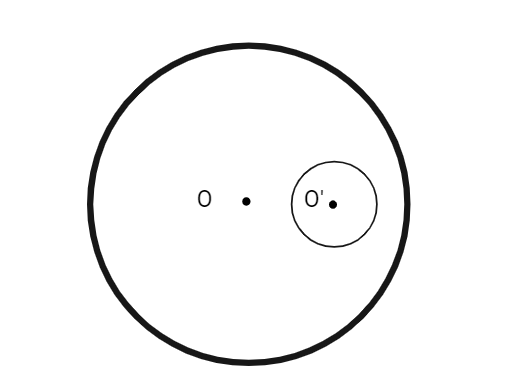
\includegraphics[width=0.4\textwidth]{lidenbrock.png}
  \label{fig:image1}
\end{figure}

\section{Calcul de champ}
On considère un fil conducteur parcouru par un courant I pénétrant dans un conducteur isotrope occupant tout l'espace des $z>0$. Déterminer le champ magnétique dans le concucteur illimité $z>0$. 
\begin{figure}[h]
  \centering
  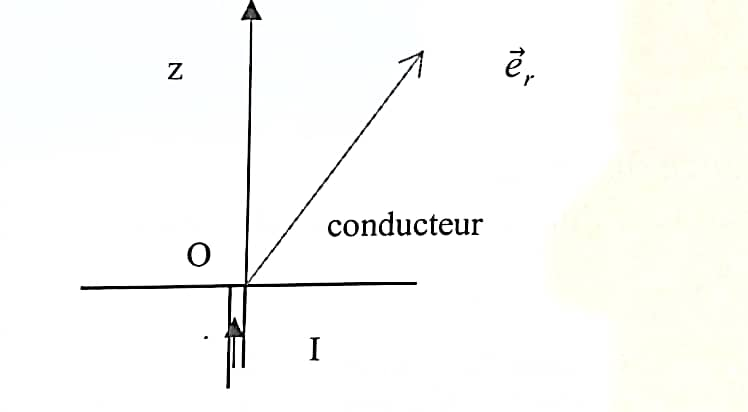
\includegraphics[width=0.4\textwidth]{schéma_conducteur_isotrope.jpg}
  \label{fig:image1}
\end{figure}

\section{L'effet de peau}
 Soit une OPPH (onde radio, $\lambda=1 cm$), se propageant selon les x croissants et rencontrant un conducteur non parfait de conductivité $\gamma$ occupant tout le demi espace $x>0$.
On note $\vec{E} = E_0 e^{i(\omega t - k x)}\vec{u_y}$ le champ électrique et $\vec{B} = B_0 e^{i(\omega t - k x)}\vec{u_z}$ le champ magnétique. 
\begin{figure}[h]
  \centering
  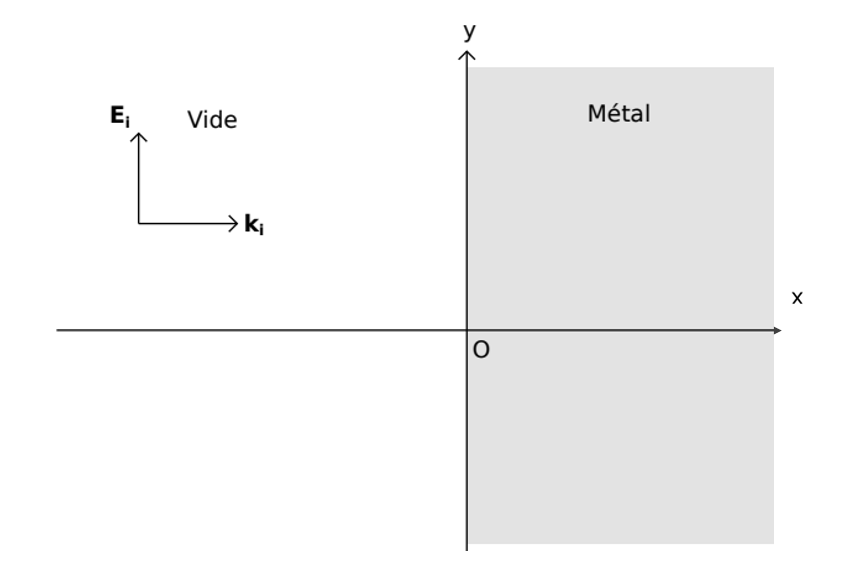
\includegraphics[width=0.4\textwidth]{schéma.png}
  \label{fig:image1}
\end{figure}
\begin {enumerate} 

\item Montrer que la densité de charge est nulle partout dans le conducteur. 
\item En supposant que $\epsilon_0 \omega << \gamma$ (approximation que l'on justifiera), montrer que l'équation de propagation d'une onde dans le conducteur s'écrit : $\vec{\Delta} \vec{E} = \mu_0 \gamma \frac{\partial\vec{E}}{\partial t}\ $
\item On cherche une onde transmise de la forme $\vec{E_t}=\vec{E_{t0}} e^{i(\omega t - k_t x)}$. Calculer $k_t$ puis expliciter la forme de l'onde transmise.
\end {enumerate} 

\end{document}



\section{Exercice 1}

\section{Exercice 2}

\section{Exercice 3}

\section{ Formulaire }

\end{document}